\makepart{Deep Learning in Action: From Neural Networks to Transformer Models}


\begin{frame}
	Now that we have an understanding of the training procedure for Artificial Neural Networks, we shall examine several widely-utilized structures within the literature of Neural Networks, including Convolutional Neural Networks (CNN),Resdiual Networks (ResNet),  Recurrent Neural Networks (RNN), and Transformers.
\end{frame}

\section{Convolutional Neural Networks}
\begin{frame}
	In the field of image processing, the Convolution Operators are widely considered as the most favoured approach. While it has been demonstrated that Dense blocks, or Linear blocks, are capable of accurately classifying images in the case of the MNIST dataset, the need for convolutional transformations arises when addressing wider and more intricate datasets.
\end{frame}
\subsection{The Two dimensional Convolution}
\begin{frame}
	A 2D convolution in a neural network context can be mathematically represented as a sliding window operation where a filter (also called kernel) $w$ of size $k \times k$ is applied to each $k \times k$ sub-matrix of the input matrix $x$. The operation can be defined as the element-wise multiplication of the filter $w$ and the sub-matrix followed by summing the results, i.e.

	$$y_{i,j} = \sum\limits_{m=1}^{k} \sum\limits_{n}^{k} w_{m,n} \cdot x_{i+m, j+n}$$

	\begin{figure}
		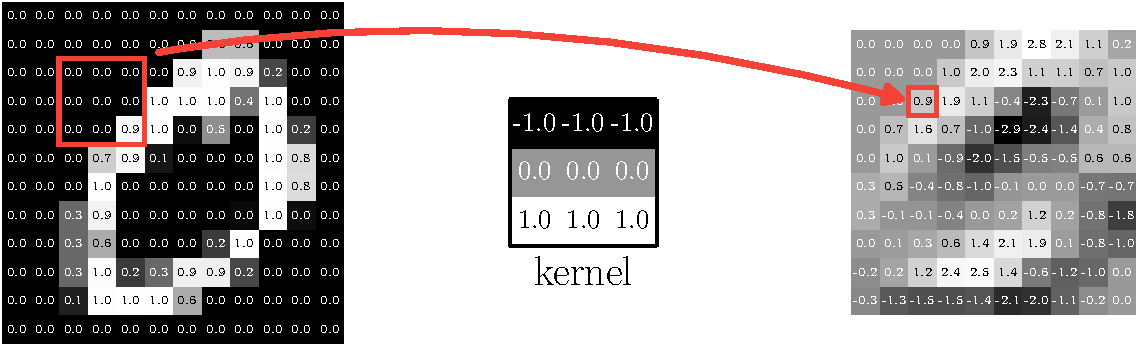
\includegraphics[width=0.6\textwidth]{figures/conv1.pdf}
	\end{figure}
\end{frame}


\begin{frame}
	A 2D convolution in a neural network context can be mathematically represented as a sliding window operation where a filter (also called kernel) $w$ of size $k \times k$ is applied to each $k \times k$ submatrix of the input matrix $x$. The operation can be defined as the element-wise multiplication of the filter $w$ and the submatrix followed by summing the results, i.e.

	$$y_{i,j} = \sum\limits_{m=1}^{k} \sum\limits_{n}^{k} w_{m,n} \cdot x_{i+m, j+n}$$

	\begin{figure}
		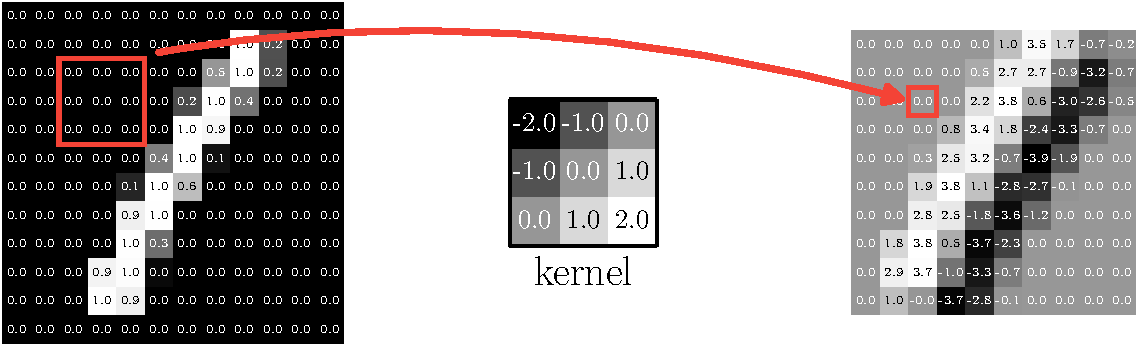
\includegraphics[width=0.6\textwidth]{figures/conv2.pdf}
	\end{figure}
\end{frame}
\begin{frame}{}{Kernel Size, Padding and  Stride}
	In every Deep Learning library, the Conv2D block takes three parameters in argument:
	\begin{itemize}
		\item the Kernel's size,
		\item the Stride,
		\item the Padding.
	\end{itemize}
	The size out the output is :
	$$
		d_{\mathrm{out}} = \frac{d_{\mathrm{in}}+2\times \mathrm{Padding}  - \mathrm{Kernel Size}  }{\mathrm{Stride}}+1
	$$
\end{frame}

\begin{frame}{}{Kernel Size, Padding and  Stride}
	Kernel size: $3$, Padding: $0$, Stride: $1$
	\begin{figure}
		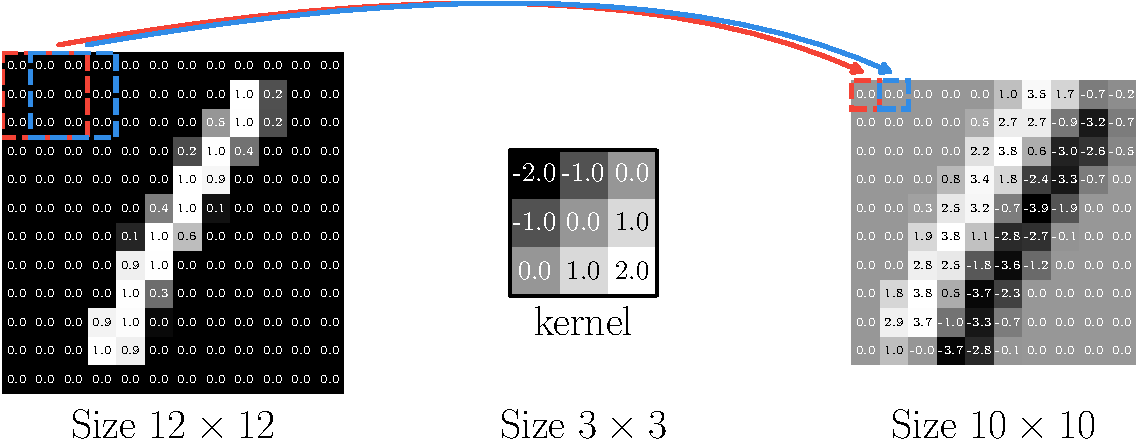
\includegraphics[width = 0.7 \textwidth]{figures/convk3.pdf}
	\end{figure}
	\vfill
	$$
		d_{\mathrm{out}} = \frac{d_{\mathrm{in}}+2\times \mathrm{Padding}  - \mathrm{Kernel Size}  }{\mathrm{Stride}}+1
	$$
\end{frame}

\begin{frame}{}{Kernel Size, Padding and  Stride}
	Kernel size: $5$, Padding: $0$, Stride: $1$
	\begin{figure}
		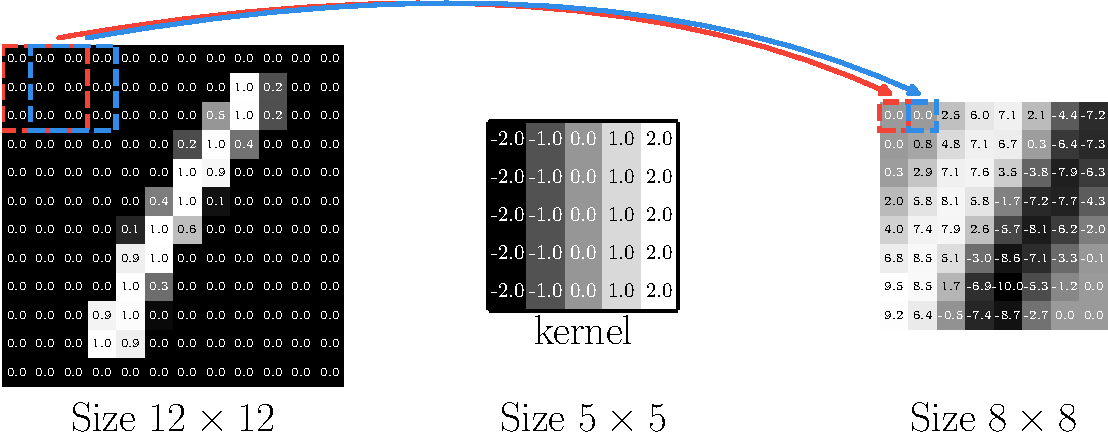
\includegraphics[width = 0.7 \textwidth]{figures/convk5.pdf}
	\end{figure}
	\vfill
	$$
		d_{\mathrm{out}} = \frac{d_{\mathrm{in}}+2\times \mathrm{Padding}  - \mathrm{Kernel Size}  }{\mathrm{Stride}}+1
	$$
\end{frame}

\begin{frame}{}{Kernel Size, Padding and  Stride}
	Kernel size: $3$, Padding: $1$, Stride: $1$. Padding mode can be 'zeros', 'reflect', 'replicate' or 'circular'.
	\begin{figure}
		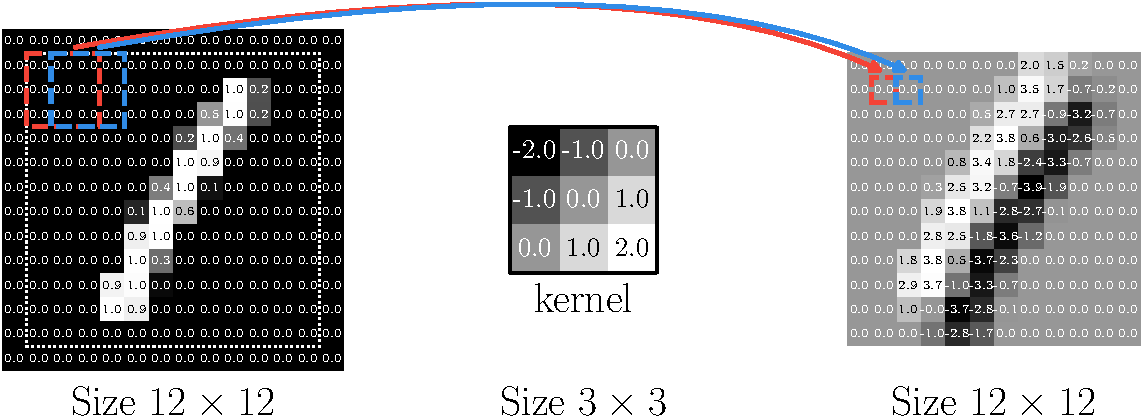
\includegraphics[width = 0.7 \textwidth]{figures/convp1.pdf}
	\end{figure}
	\vfill
	$$
		d_{\mathrm{out}} = \frac{d_{\mathrm{in}}+2\times \mathrm{Padding}  - \mathrm{Kernel Size}  }{\mathrm{Stride}}+1
	$$
\end{frame}

\begin{frame}{}{Kernel Size, Padding and  Stride}
	Kernel size: $3$, Padding: $1$, Stride: $2$
	\begin{figure}
		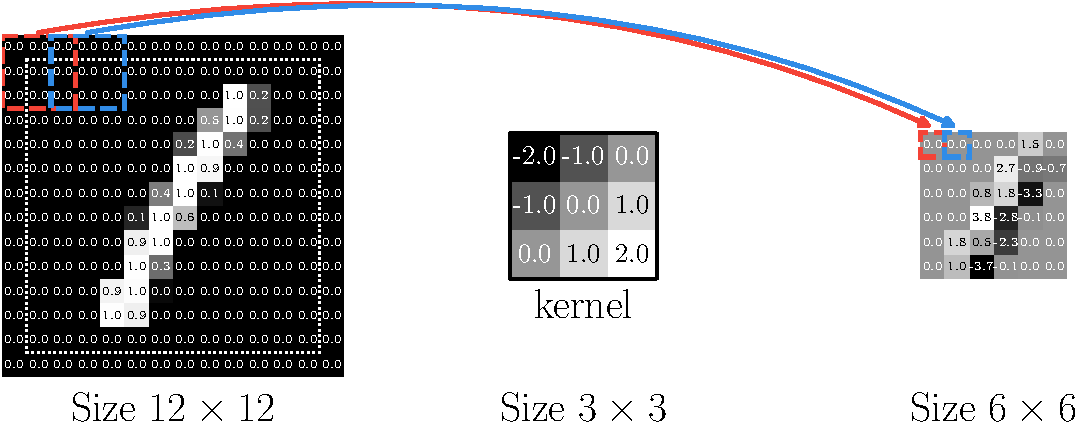
\includegraphics[width = 0.7 \textwidth]{figures/convs2.pdf}
	\end{figure}
	\vfill
	$$
		d_{\mathrm{out}} = \frac{d_{\mathrm{in}}+2\times \mathrm{Padding}  - \mathrm{Kernel Size}  }{\mathrm{Stride}}+1
	$$
\end{frame}

\begin{frame}{}{Kernel Size, Padding and  Stride}
	Kernel size: $3$, Padding: $1$, Stride: $3$
	\begin{figure}
		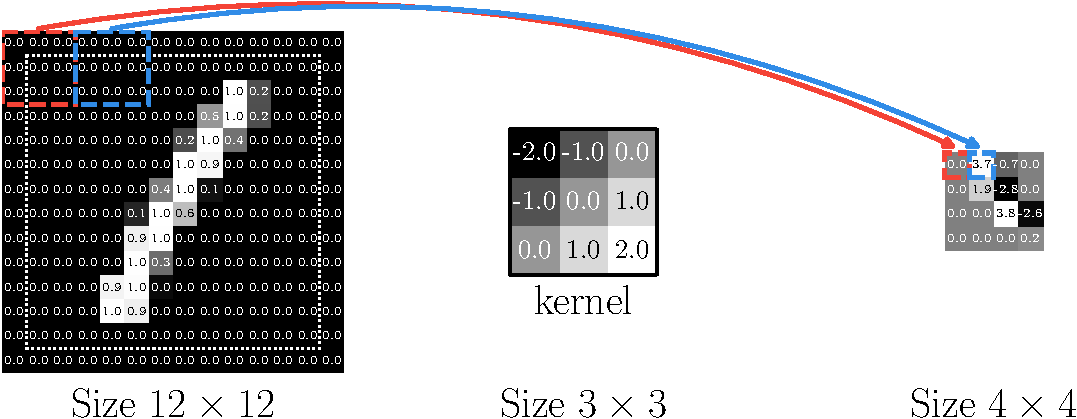
\includegraphics[width = 0.7 \textwidth]{figures/convs3.pdf}
	\end{figure}
	\vfill
	$$
		d_{\mathrm{out}} = \frac{d_{\mathrm{in}}+2\times \mathrm{Padding}  - \mathrm{Kernel Size}  }{\mathrm{Stride}}+1
	$$
\end{frame}

\subsection{CNN : Convolutional in a network Networks}
\begin{frame}
	We can  represent a CNN as under this form:

	\begin{figure}
		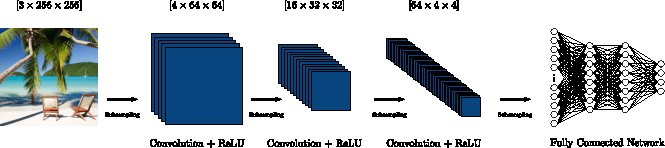
\includegraphics[width=1\textwidth]{figures/conv.pdf}
	\end{figure}
\end{frame}

\begin{frame}
	Usually, the output of a convolutional block is linear combination of the Convolutional output of every previous channels and a bias:
	$$
		\mathrm{out}_{i,j}(c_\mathrm{out}) = \mathrm{bias}(c_\mathrm{out}) + \sum_{k=0}^{\vert c_{\mathrm{in}} \vert-1} \mathrm{Conv}(\mathrm{input}(k), \mathrm{kernel}_k )_{i,j}
	$$

	\begin{figure}
		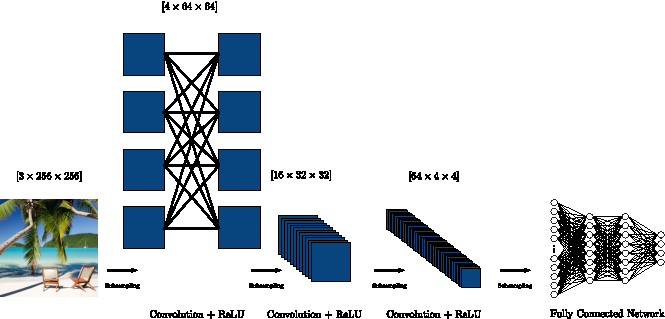
\includegraphics[width=0.7\textwidth]{figures/convfc1.pdf}
	\end{figure}

\end{frame}

\begin{frame}
	In practice, we split the image into multiple channels : the three channels RGB to begin with. Then we apply convolutional operation on different scales and then we use a fully connected tail. To change the scale we can use different sub-sampling : Max pooling, Average pooling or Invertible pooling.

	\begin{figure}
		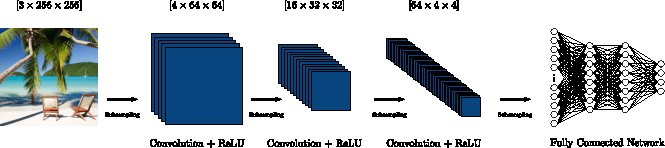
\includegraphics[width=1\textwidth]{figures/conv.pdf}
	\end{figure}
\end{frame}

\begin{frame}{}{Max Pooling}
	Max Pooling take the maximum within a given sized sub-matrix. In practice, the matrix is size $2\times 2$ in order to reduce the dimension by $4$ and doubling the scale.

	\begin{figure}
		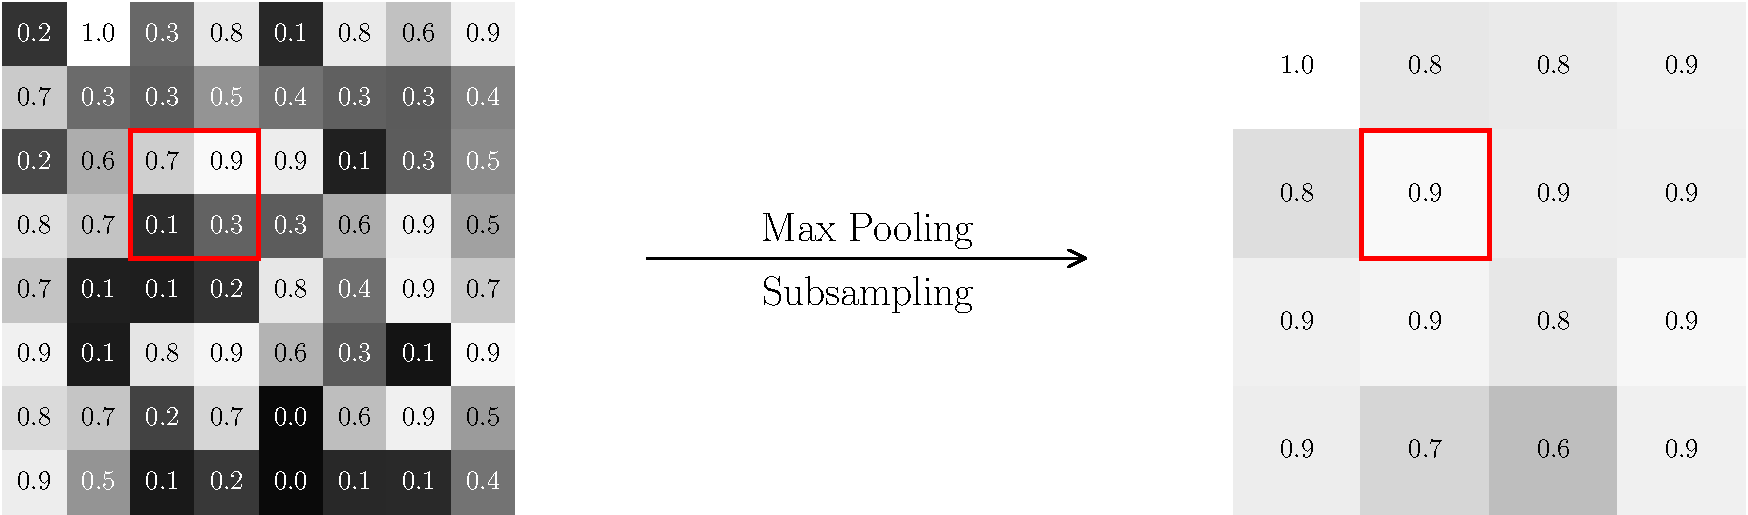
\includegraphics[width=1\textwidth]{figures/maxpooling.pdf}
	\end{figure}
\end{frame}


\begin{frame}{}{Average Pooling}
	The Average pooling takes the average value within the sub-matrix.

	\begin{figure}
		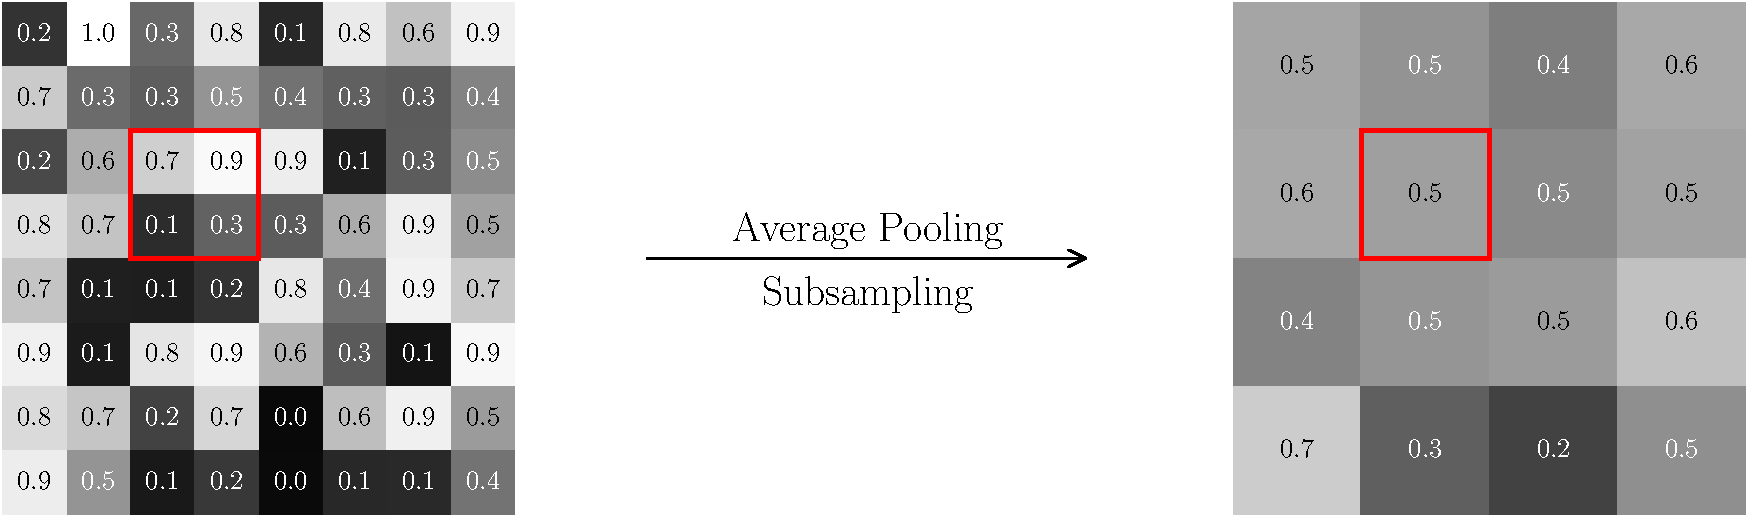
\includegraphics[width=1\textwidth]{figures/avgpooling.pdf}
	\end{figure}
\end{frame}


\begin{frame}{}{Invertible Pooling}
	For Invertible Networks, we can use Invertible Pooling, aka Squeeze. It preserves the information contained in the channels and keeps the dimension constant.

	\begin{figure}
		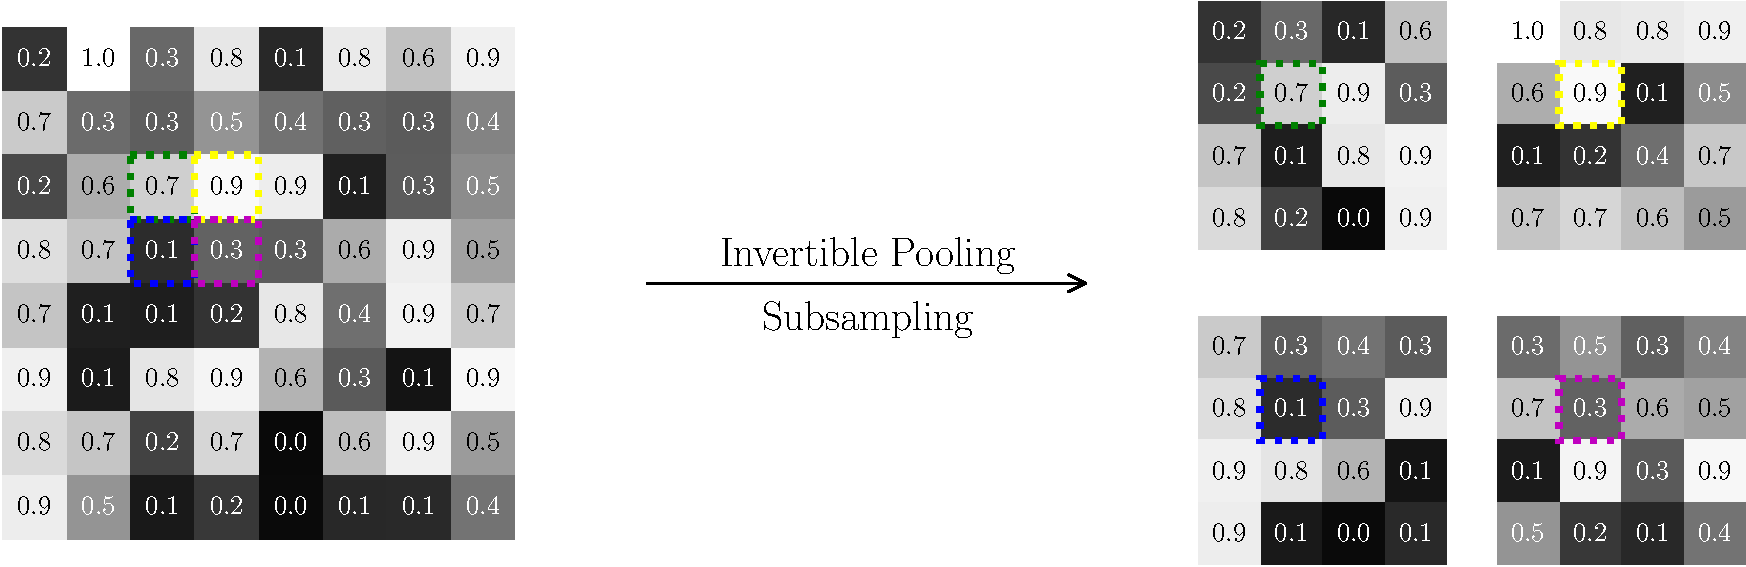
\includegraphics[width=1\textwidth]{figures/squeezepooling.pdf}
	\end{figure}
\end{frame}


\begin{frame}
	Convolutional Neural Networks are more suitable for image processing compared to fully connected networks due to their ability to efficiently handle the spatial relationships between pixels in an image. This is achieved through the use of convolutional layers that apply filters to small portions of an image, rather than fully connected layers that process the entire image as a single vector. Additionally, the shared weights in convolutional layers allow for learning of hierarchical features, reducing the number of parameters in the network and increasing its ability to generalize to new images.
\end{frame}

\subsection{CNN in practice: CIFAR 10}

\begin{frame}
	\begin{itemize}
		\item Input shape : $3 \times 32 \times32$.
		\item Number of Classes : $10$.
		\item Number of training samples $(x, y)$: $50000$.
		\item Number of evaluating samples: $10000$.
	\end{itemize}
	\begin{figure}
		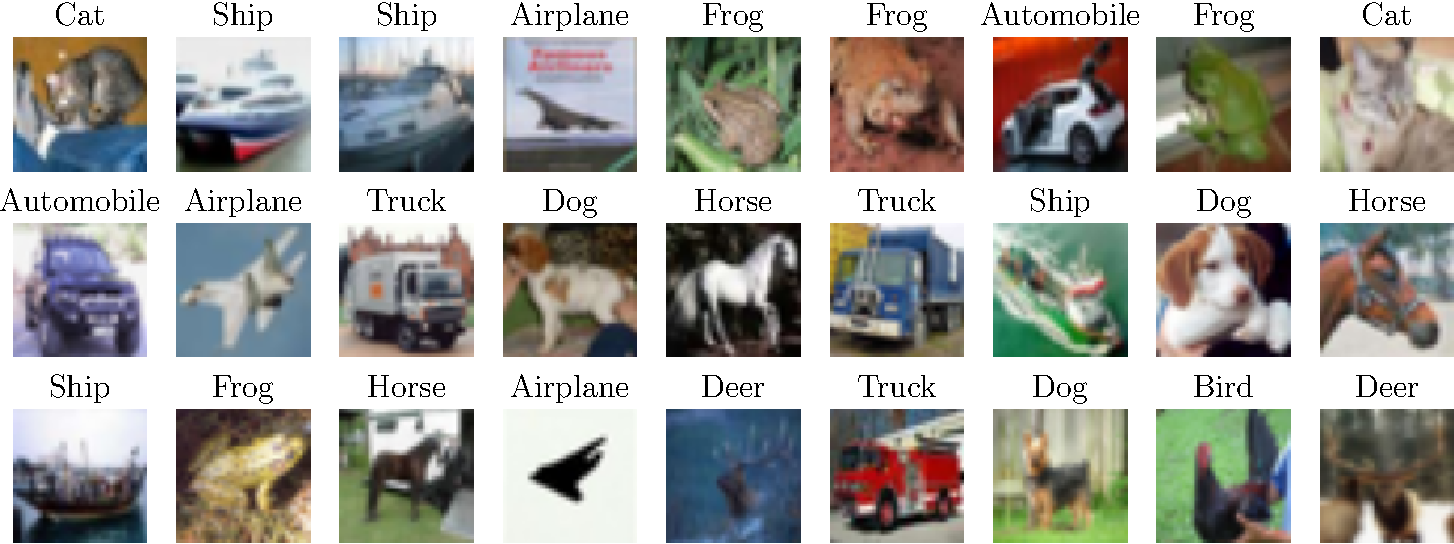
\includegraphics[width= 0.8\textwidth]{figures/cifar10.pdf}
	\end{figure}
\end{frame}
\begin{frame}
	We will compare three different models:
	\begin{itemize}

		\item Model 1 : Fully Connected Neural Network with $3.4$ million parameters.
		\item Model 2 : CNN with $62$ thousand parameters.
		\item Model 3 : Wider and longer CNN with $5.8$ million parameters.
	\end{itemize}
\end{frame}

\begin{frame}{}{Model 1 : Fully Connected Neural Network}
	The Net in composed of 4 linear layers with ReLU activations:
	\begin{itemize}
		\item Linear $3072 \mapsto 1024$ + ReLU
		\item Linear $1024 \mapsto 256$ + ReLU
		\item Linear $256 \mapsto 64$ + ReLU
		\item Linear $64 \mapsto 10$ + SoftMax
	\end{itemize}
\end{frame}

\begin{frame}{}{Model 1}
	\begin{figure}
		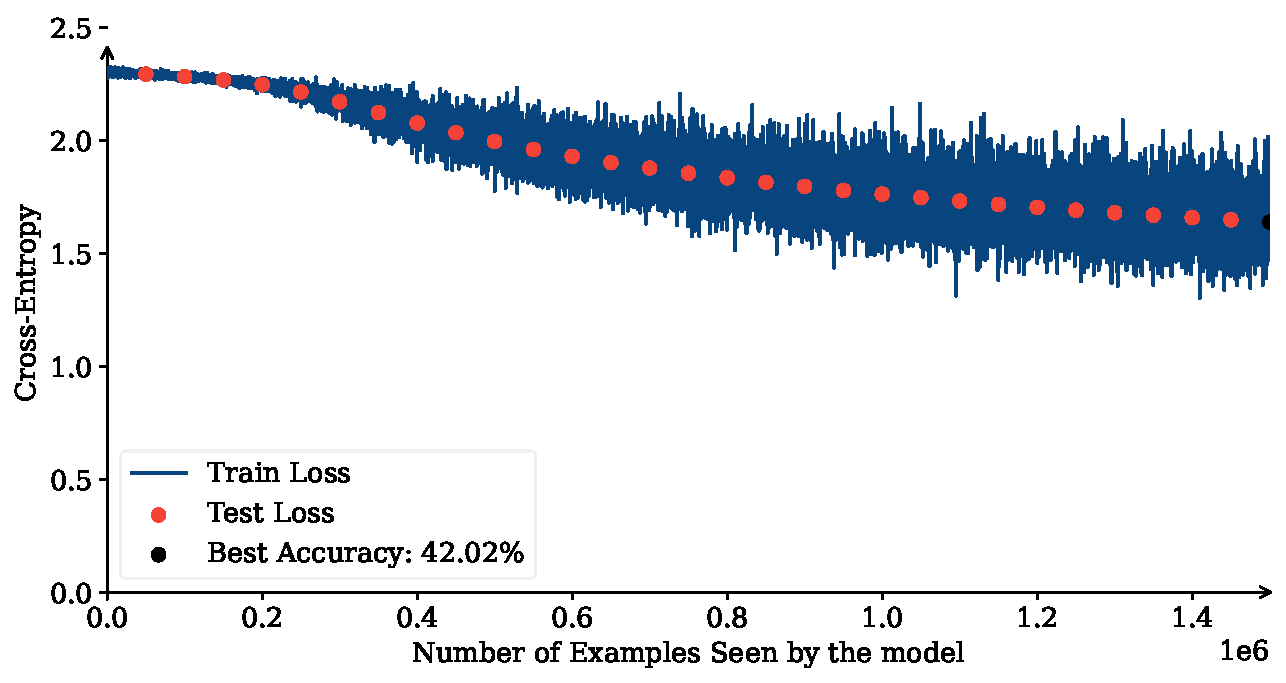
\includegraphics[width = 0.7 \textwidth]{figures/sgd_cifar_fc.pdf}
	\end{figure}
\end{frame}

\begin{frame}{}{Using a better optimization algorithm ?}
	\textbf{Adam}: Adam is an optimization algorithm that can be used instead of the classical stochastic gradient descent procedure to update network weights iteratively based on training data. It combines the advantages of two other extensions of stochastic gradient descent, AdaGrad and RMSProp, and is designed to work well for a wide range of applications:
	\begin{align*}
		\theta_{t+1} & = \theta_t - \frac{\lambda}{\sqrt{\hat{v}_t} + \varepsilon} \hat{m}_t \\
		\hat{m}_t    & = \beta_1 m_{t-1} + (1-\beta_1) \nabla_\theta l(\theta_t)             \\
		\hat{v}_t    & = \beta_2 v_{t-1} + (1-\beta_2) \nabla_\theta l(\theta_t)^2
	\end{align*}
	\begin{itemize}
		\item $\lambda$ is the learning rate.
		\item $\hat{m}_t$ is the moving average of the gradient. It allows to smooth the gradient step.
		\item By dividing the gradient by the square root of the moving average of the squared gradient, we can adapt the learning rate for each parameter to improve the convergence speed.
	\end{itemize}
\end{frame}


\begin{frame}{}{Model 1}
	\begin{figure}
		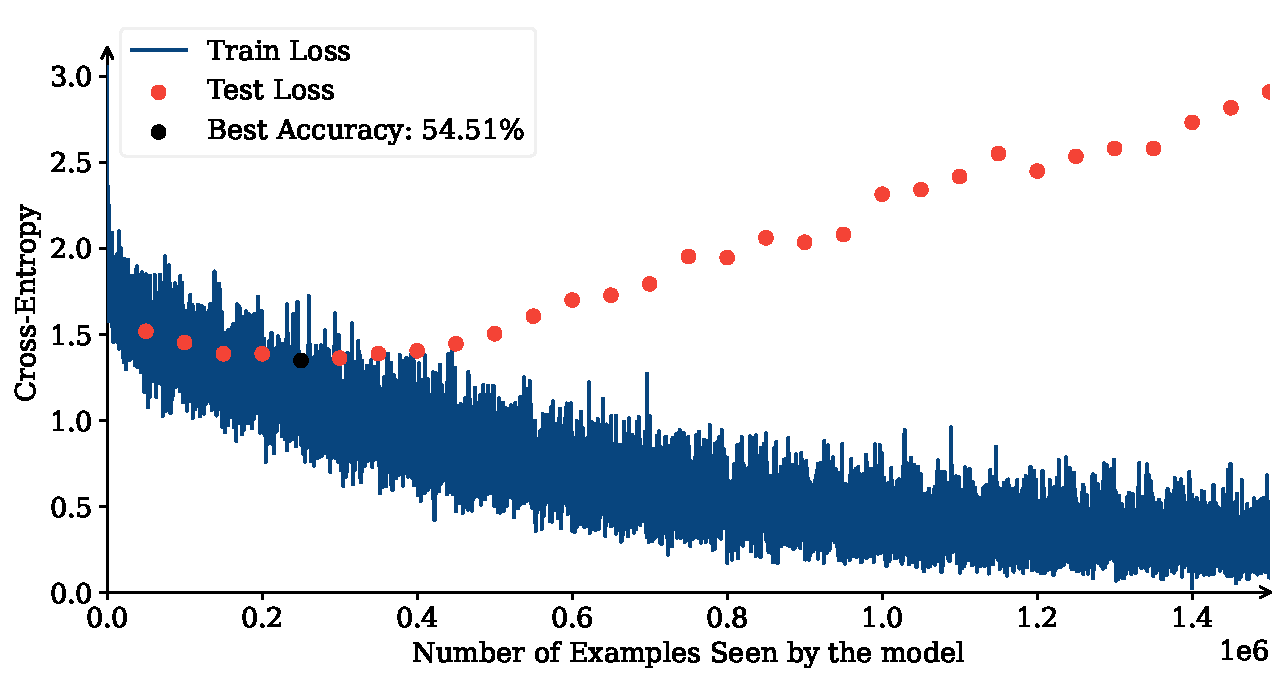
\includegraphics[width = 0.7 \textwidth]{figures/adam_cifar_fc.pdf}
	\end{figure}
\end{frame}

\begin{frame}{}{Model 1}
	\begin{figure}
		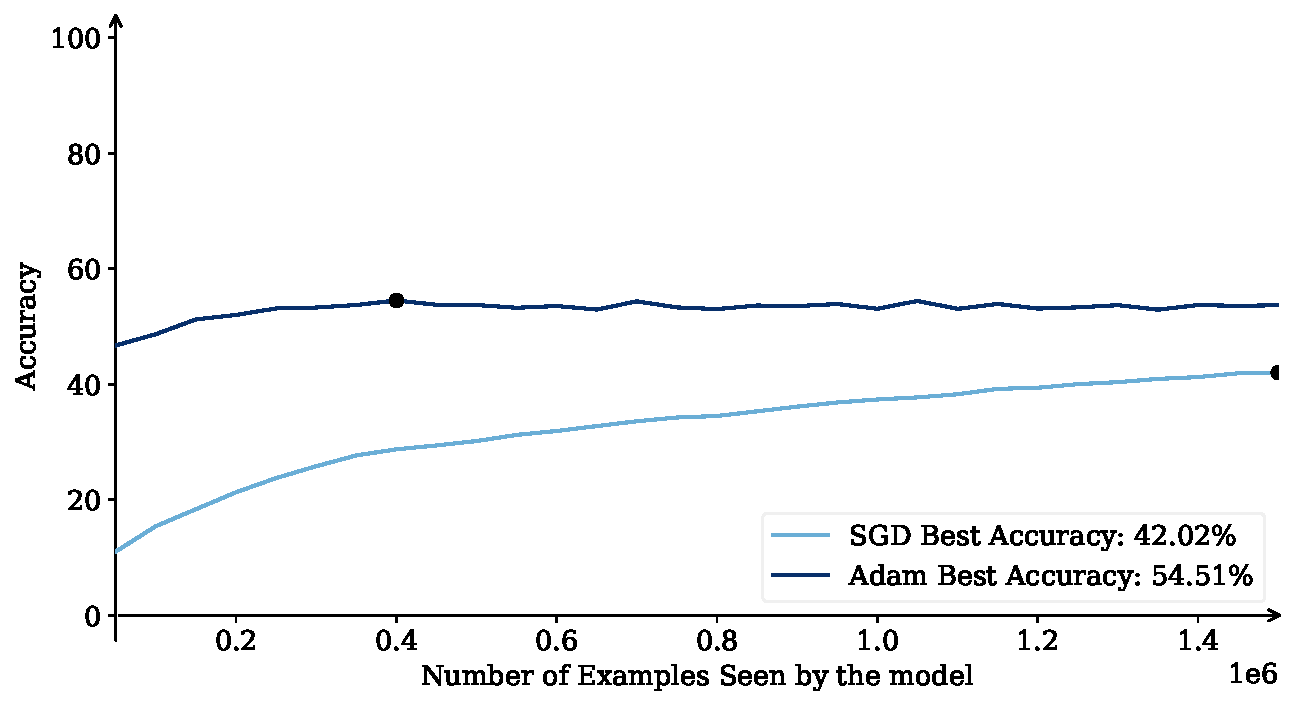
\includegraphics[width = 0.7 \textwidth]{figures/accuracies_cifar_fc.pdf}
	\end{figure}
\end{frame}

\begin{frame}{}{Model 2}
	The Net is composed 2 convolutional layers and 2 linear layers:
	\begin{itemize}
		\item Conv $3\times 32 \times 32 \mapsto 6 \times 28 \times 28$ + ReLU
		\item Max Pooling $ 6 \times 28 \times 28 \mapsto 6 \times 14 \times 14$
		\item Conv $6\times 14 \times 14 \mapsto 16 \times 10 \times 10$ + ReLU
		\item Max Pooling $ 16 \times 10 \times 10 \mapsto 16 \times 5 \times 5$
		\item Linear $400 \mapsto 120$ + ReLU
		\item Linear $120 \mapsto 84$ + ReLU
		\item Linear $84 \mapsto 10$ + SoftMax
	\end{itemize}
\end{frame}

\begin{frame}{}{Model 2}
	\begin{figure}
		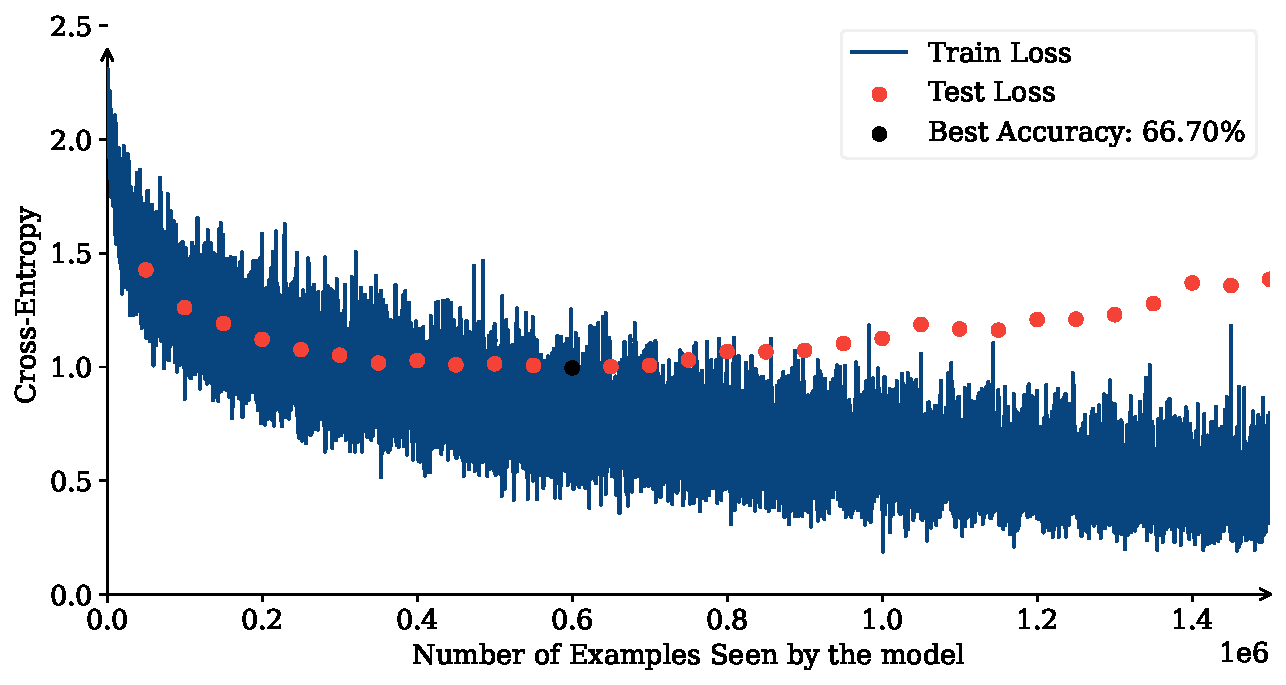
\includegraphics[width = 0.7 \textwidth]{figures/cifar_cnn.pdf}
	\end{figure}
\end{frame}



\begin{frame}{}{Model 3}

	The Net is composed 6 convolutional layers and 3 linear layers:
	\begin{itemize}
		\item Conv $3\times 32 \times 32 \mapsto 32 \times 32 \times 32$ + BatchNorm2d + ReLU
		\item Conv $32\times 32 \times 32 \mapsto 64 \times 32 \times 32$ + ReLU
		\item Max Pooling $ 64 \times 32 \times 32 \mapsto 64 \times 16 \times 16$
		\item Conv $64\times 16 \times 16 \mapsto 128 \times 16 \times 16$ + BatchNorm2d + ReLU
		\item Conv $128\times 16 \times 16 \mapsto 128 \times 16 \times 16$ + ReLU
		\item Max Pooling $ 128 \times 16 \times 16 \mapsto 128 \times 8 \times 8$
		\item Conv $128\times 8 \times 8 \mapsto 256 \times 8 \times 8$ + BatchNorm2d + ReLU
		\item Conv $256\times 8 \times 8 \mapsto 256 \times 8 \times 8$ + ReLU
		\item Max Pooling $ 256 \times 8 \times 8 \mapsto 256 \times 4 \times 4$ + DropOut $p=0.05$
		\item Linear $4096 \mapsto 1024$ + ReLU
		\item Linear $1024 \mapsto 512$ + ReLU + DropOut $p=0.05$
		\item Linear $512 \mapsto 10$ + SoftMax
	\end{itemize}
	We have added Batch Normalization to improve the training stability and Drop Out to reduce overfitting.
\end{frame}

\begin{frame}{}{Model 3 without Batch Normalization and Drop Out}
	\begin{figure}
		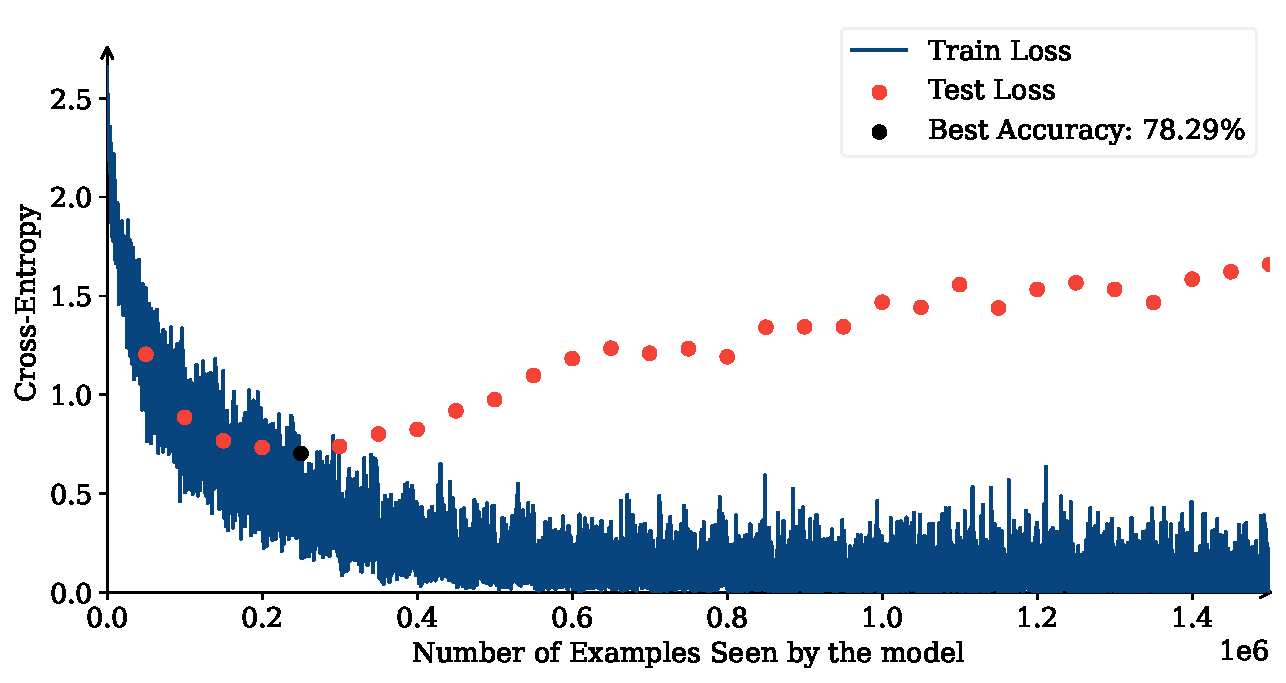
\includegraphics[width = 0.7 \textwidth]{figures/cifar_large_cnn.pdf}
	\end{figure}
\end{frame}

\begin{frame}{}{Batch Normalization}
	Batch normalization is used to normalize the activations of a layer within a batch of data.
	\begin{itemize}
		\item This helps to prevent the problem of vanishing or exploding gradients and also speeds up the training process.
		\item 	By normalizing the activations, batch normalization helps to stabilize the distribution of the inputs to each layer, reducing the covariate shift and allowing the network to learn more effectively.
	\end{itemize}


\end{frame}

\begin{frame}{}{Batch Normalization}
	\begin{small}
		\begin{algorithm}[H]
			\caption{Batch Normalization during training}
			\begin{algorithmic}[1]
				\FOR{each $x_i$ in a mini-batch $B$ of size $b$}
				\STATE Compute the mean $\mu_B$ and variance $\sigma_B^2$ of the features in the mini-batch $B$.
				$$\mu_B = \frac{1}{b}\sum_ix_i \quad \mbox{and} \quad\sigma_B^2=\frac{1}{m}\sum_i\left(x_i-\mu_B\right)^2 $$
				\STATE Normalize each feature $x_i$ in the mini-batch $B$ using $\mu_B$ and $\sigma_B^2$.
				$$\bar x_i = \frac{x_i-\mu_B}{\sqrt{\sigma_B^2 + \varepsilon}} $$
				\STATE Scale and shift each normalized feature $x_i$ using two learnable parameters $\gamma$ and $\beta$ respectively.
				$$ y_i = \gamma \bar x_i + \beta $$
				\STATE Update the moving average of the mean and variance for inference:
				$$
					\mu = (1-\gamma)\mu + \gamma \mu_B \quad \mbox{and} \quad \sigma^2 = (1-\gamma)\sigma^2 + \gamma \sigma_B^2 $$
				\ENDFOR
			\end{algorithmic}
		\end{algorithm}
	\end{small}
\end{frame}

\begin{frame}{}{Batch Normalization}
	At inference:
	\begin{algorithm}[H]
		\caption{Batch Normalization at inference}
		\begin{algorithmic}[1]
			\FOR{each $x_i$}
			\STATE Normalize each feature $x_i$ using the moving average of the mean and variance:
			$$\bar x_i = \frac{x_i-\mu}{\sqrt{\sigma^2 + \varepsilon}} $$
			\STATE Scale and shift each normalized feature $x_i$ using two learnable parameters $\gamma$ and $\beta$ respectively.
			$$ y_i = \gamma \bar x_i + \beta $$
			\ENDFOR
		\end{algorithmic}
	\end{algorithm}
\end{frame}

\begin{frame}{}{Model 3 without Drop Out}
	\begin{figure}
		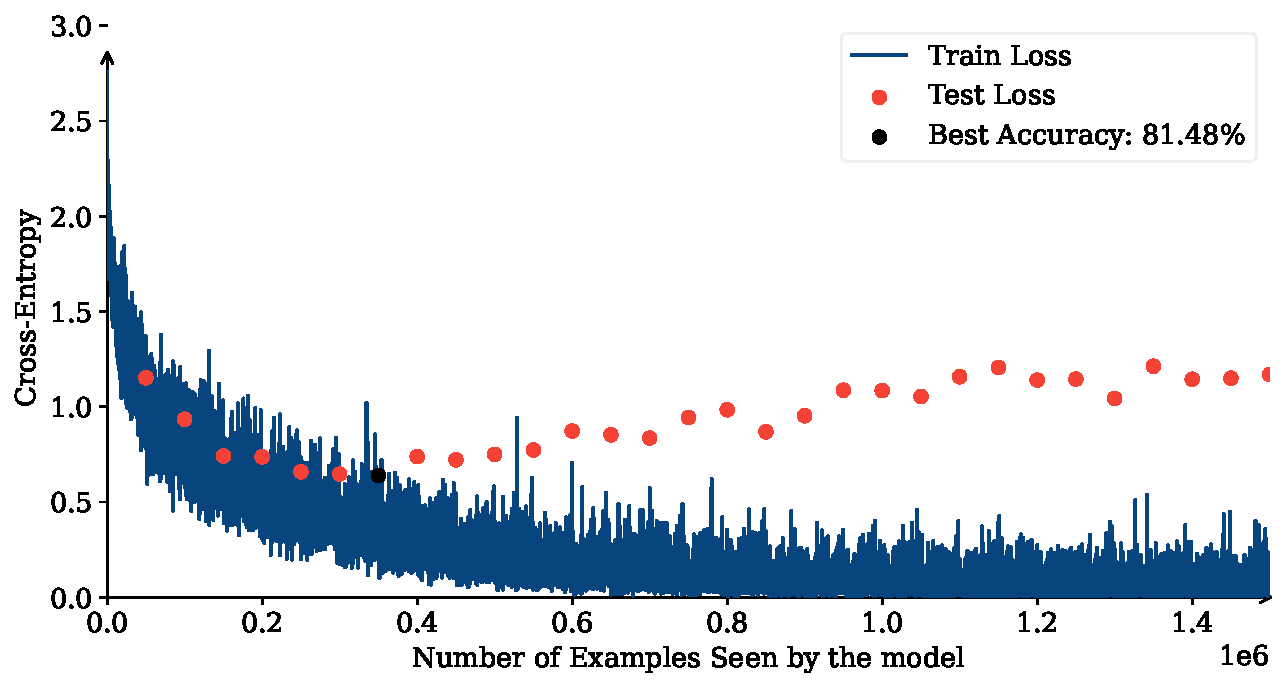
\includegraphics[width = 0.7 \textwidth]{figures/cifar_large_cnn_bn.pdf}
	\end{figure}
\end{frame}


\begin{frame}{}{Drop out}
	Dropout is a regularization technique in neural networks where \alert{during training}, a portion of the nodes are randomly "dropped out" or ignored during each iteration. This helps prevent over-fitting by preventing the model from relying too heavily on any one node. The result is a more robust and generalizable model that can better handle unseen data.
	\begin{figure}
		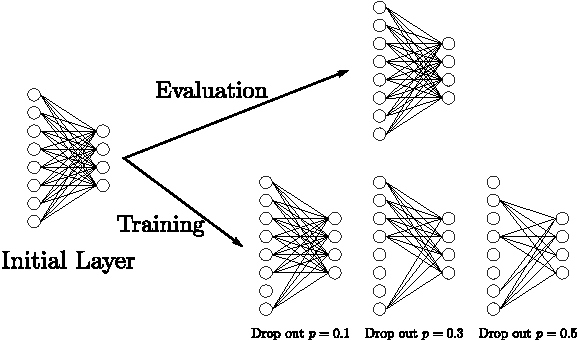
\includegraphics[width=0.7\textwidth]{figures/dropout.pdf}
	\end{figure}
\end{frame}

\begin{frame}{}{Model 3}
	\begin{figure}
		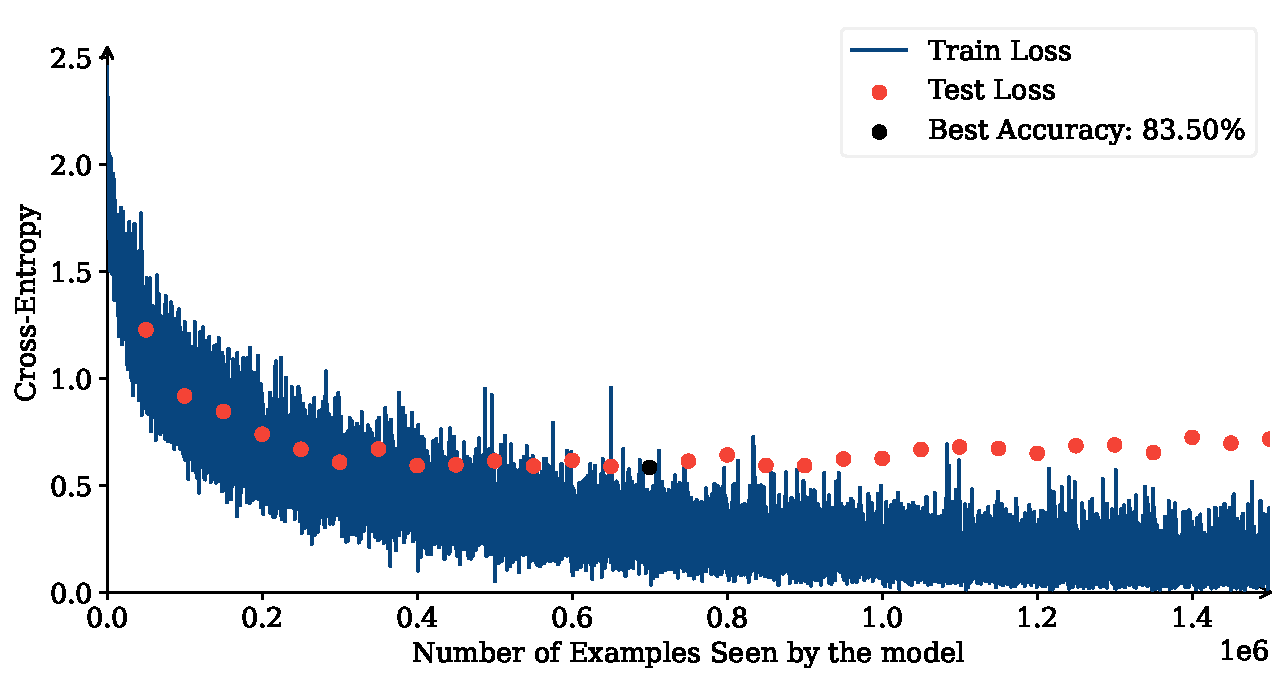
\includegraphics[width = 0.7 \textwidth]{figures/cifar_large_cnn_bn_dropout.pdf}
	\end{figure}
\end{frame}

\begin{frame}{}{Model 3}
	\begin{figure}
		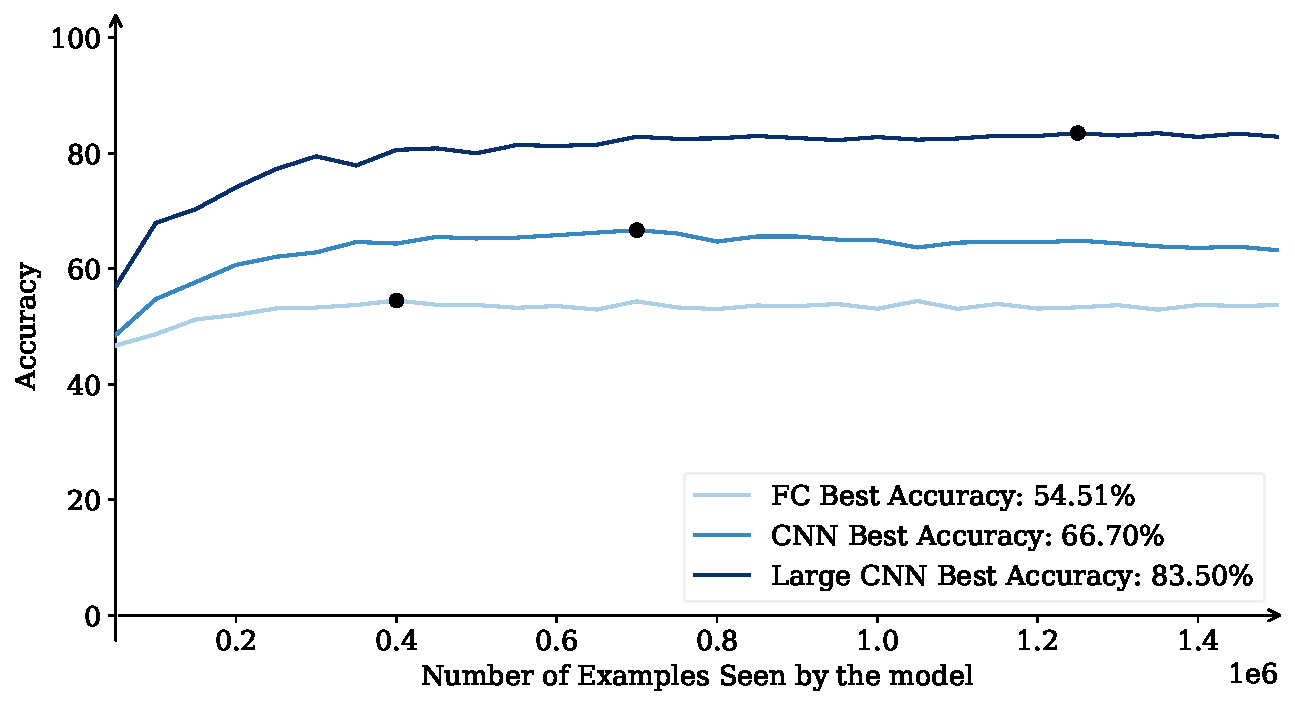
\includegraphics[width = 0.7 \textwidth]{figures/accuracies_cifar_cnn.pdf}
	\end{figure}
\end{frame}

\begin{frame}
	\begin{figure}
		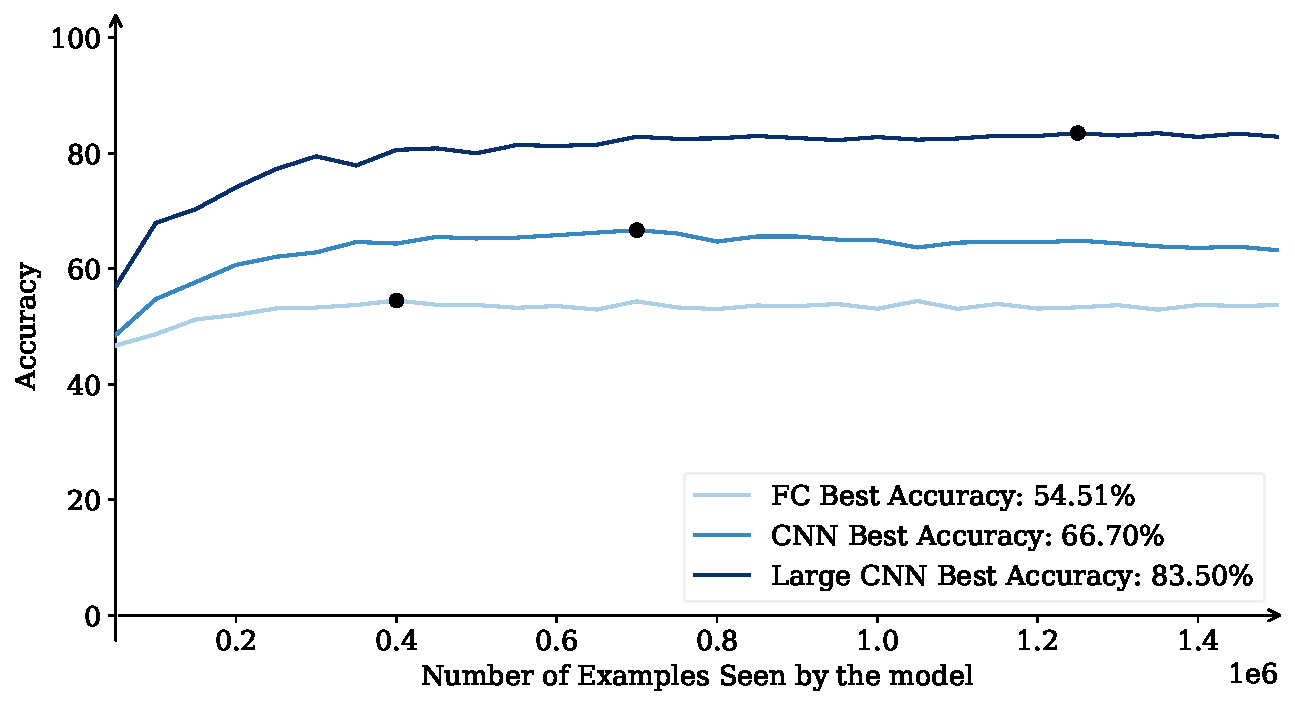
\includegraphics[width = 0.7 \textwidth]{figures/accuracies_cifar_fc_cnn.pdf}
	\end{figure}
\end{frame}

\begin{frame}{}{Intuition behind channels}
	To examine the information captured by different channels in a Neural Network, we can compare their output on a dataset. For a given input $x$, we can compute the similarity between the output of a specific channel and the same channel for other images in the dataset.
	\begin{figure}
		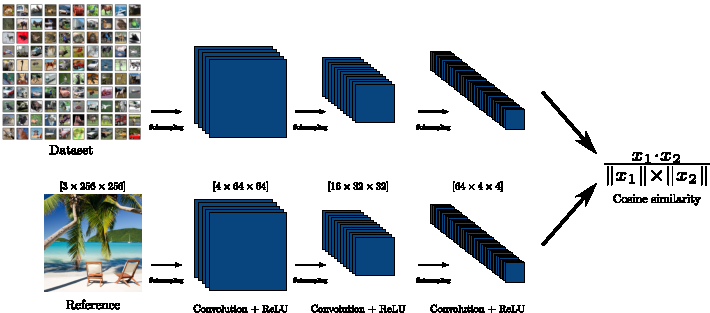
\includegraphics[width = 0.8 \textwidth]{figures/Cosine_channels.pdf}
	\end{figure}
\end{frame}
\begin{frame}{}{Intuition behind channels}
	\begin{figure}
		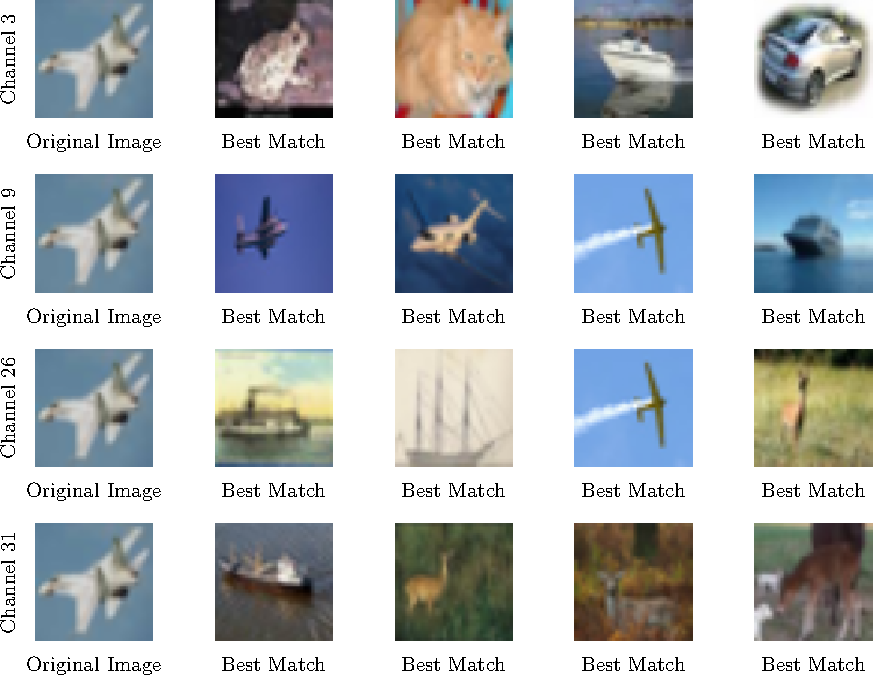
\includegraphics[width = 0.6 \textwidth]{figures/cifar10avion.pdf}
	\end{figure}
\end{frame}

\begin{frame}{}{Intuition behind channels}
	\begin{figure}
		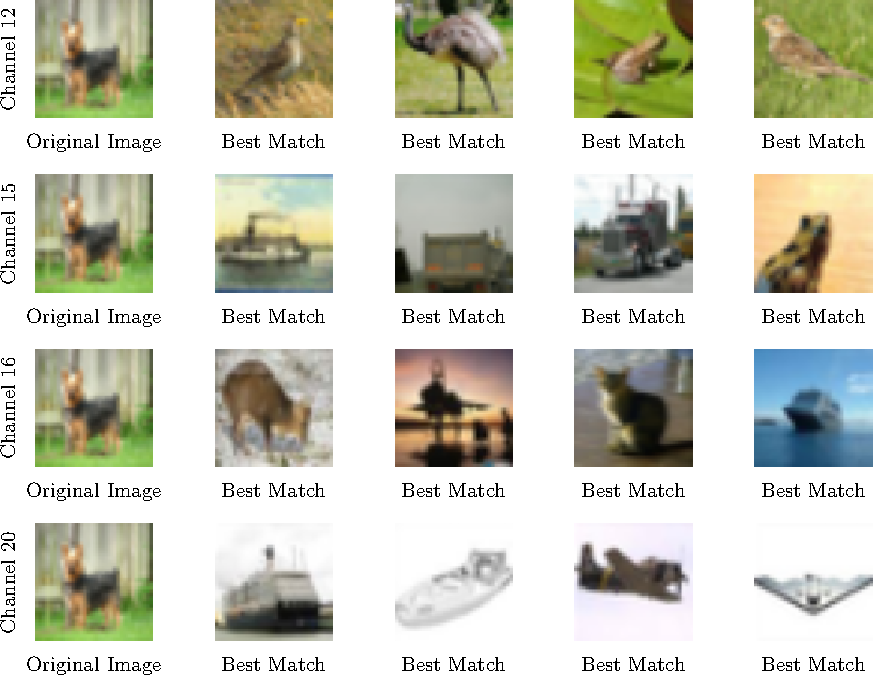
\includegraphics[width = 0.6 \textwidth]{figures/cifar10caniche.pdf}
	\end{figure}
\end{frame}
\begin{frame}{}{Intuition behind channels}
	\begin{figure}
		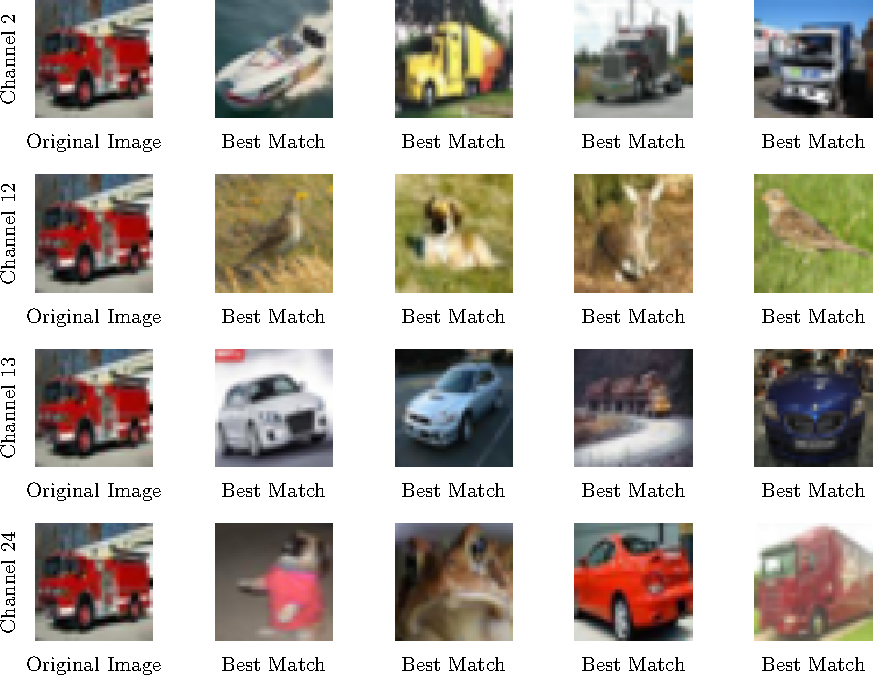
\includegraphics[width = 0.6 \textwidth]{figures/cifar10camion.pdf}
	\end{figure}
\end{frame}
\begin{frame}{}{Intuition behind channels}
	\begin{figure}
		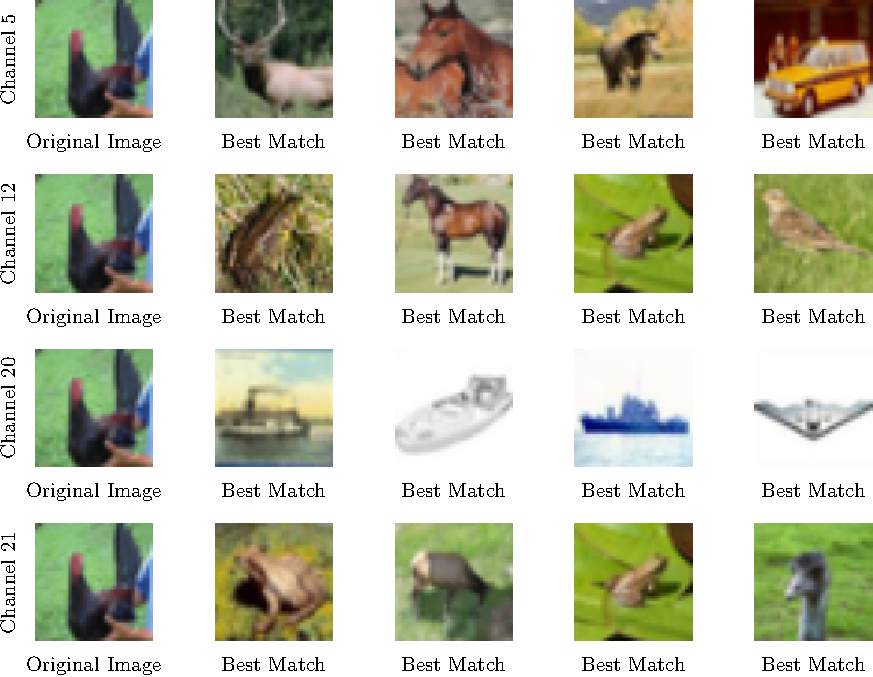
\includegraphics[width = 0.6 \textwidth]{figures/cifar10poulet.pdf}
	\end{figure}
\end{frame}


\begin{frame}{TP2: The Convolutional Neural Network}{Introduction to CNN and CIFAR-10 dataset}
	Link to the notebook (ipynb): \href{
		https://lamsade.dauphine.fr/~averine/EM_IASD/TP2.ipynb}{TP2.ipynb}\\
	Link to the notebook (html): \href{run:../notebook_pedagogiques/CNN.html}{CNN.html}
\end{frame}

\section{Recurrent Neural Networks}
\begin{frame}
	Recurrent Networks (RNNs) are a type of neural network that are specifically designed to handle sequential data, whereas CNNs are more suited for image and grid-like data. The main difference between RNNs and CNNs lies in the way they process data, with RNNs considering the sequence of elements and their interdependencies, while CNNs focus on capturing local patterns within the input.
\end{frame}

\subsection{Recurrent Block}

\begin{frame}
	A  Recurrent Network  is a type of neural network that contains a loop mechanism, allowing previous outputs to be used as inputs for future computations. This creates a form of memory that allows the network to process sequential data with variable-length sequences.
	\begin{figure}
		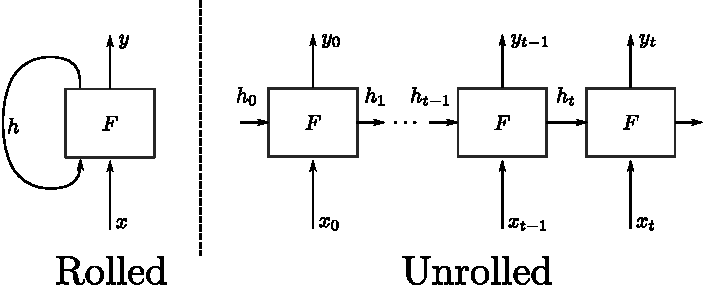
\includegraphics[width=0.7\textwidth]{figures/RNN.pdf}
	\end{figure}
\end{frame}
\begin{frame}
	\begin{columns}[c, onlytextwidth]
		\column{0.7\textwidth}
		Some of the limitations of Vanilla RNNs:
		\begin{itemize}
			\item Vanishing gradient problem: The gradient signals used to update the weights during training can become very small, making it difficult to train RNNs effectively.

			\item Exploding gradient problem: On the other hand, gradients can become too large and cause numeric instability, making it difficult to train RNNs effectively.

			\item Short-term memory: Vanilla RNNs have difficulty retaining information over long periods of time, making them unsuitable for tasks that require remembering information from previous time steps.

			\item Computational limitations: RNNs can be computationally intensive, making it difficult to apply them to large sequences of data.

			\item Difficulty with parallelization: The sequential nature of RNNs can make it difficult to take advantage of parallel processing to speed up training and inference.
		\end{itemize}
		\column{0.3\textwidth}
		\begin{figure}
			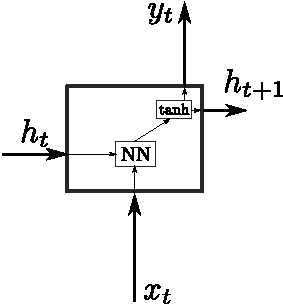
\includegraphics[width=0.8\textwidth]{figures/RNN_NN.pdf}
		\end{figure}
	\end{columns}
\end{frame}

\subsection{LSTM  and GRU}
\begin{frame}{}{LSTM}
	Long Short-Term Memory (LSTM) networks are a variant of recurrent neural networks (RNNs) that overcome some of the limitations of traditional RNNs, such as the vanishing gradient problem and difficulty in learning long-term dependencies. LSTM networks introduce memory cells, gates, and a process for updating cells, which allows them to selectively preserve information from previous time steps.

	\begin{figure}
		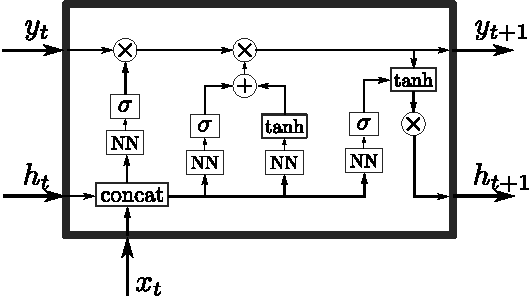
\includegraphics[width=0.7\textwidth]{figures/LSTM.pdf}
	\end{figure}
\end{frame}

\begin{frame}{}{LSTM}
	Long Short-Term Memory (LSTM) networks are a variant of recurrent neural networks (RNNs) that overcome some of the limitations of traditional RNNs, such as the problem of vanishing gradients and the difficulty of learning long-term dependencies. LSTM networks introduce memory cells, gates, and a process for updating cells, which allows them to selectively preserve information from previous time steps.

	\begin{figure}
		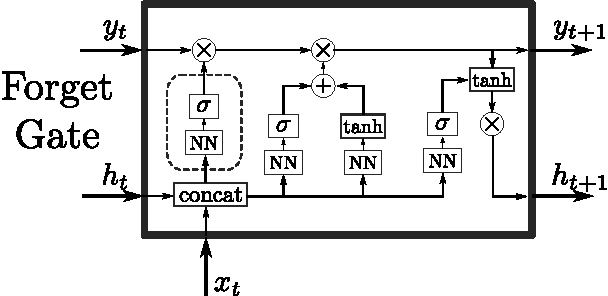
\includegraphics[width=0.6\textwidth]{figures/LSTM_forget.pdf}
	\end{figure}
\end{frame}
\begin{frame}{}{LSTM}
	Long Short-Term Memory (LSTM) networks are a variant of recurrent neural networks (RNNs) that overcome some of the limitations of traditional RNNs, such as the vanishing gradient problem and difficulty in learning long-term dependencies. LSTM networks introduce memory cells, gates, and a process for updating the cells, which allows them to selectively preserve information from previous time steps.

	\begin{figure}
		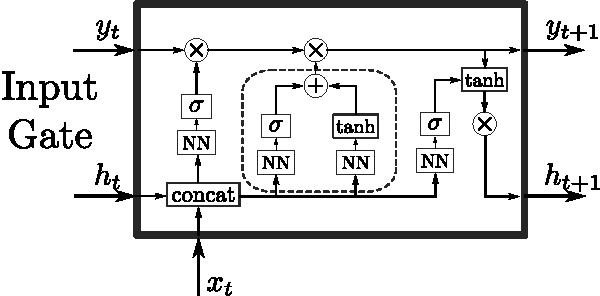
\includegraphics[width=0.6\textwidth]{figures/LSTM_input.pdf}
	\end{figure}
\end{frame}
\begin{frame}{}{LSTM}
	Long Short-Term Memory (LSTM) networks are a variant of recurrent neural networks (RNNs) that overcome some of the limitations of traditional RNNs, such as the vanishing gradient problem and difficulty in learning long-term dependencies. LSTM networks introduce memory cells, gates, and a process for updating the cells, which allows them to selectively preserve information from previous time steps.

	\begin{figure}
		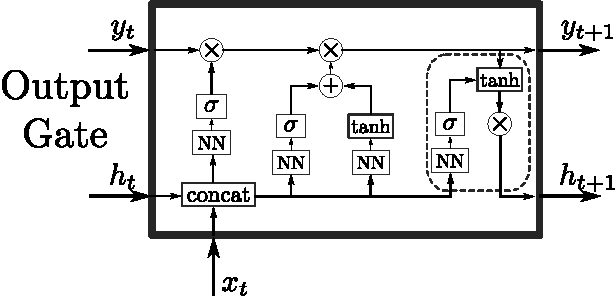
\includegraphics[width=0.6\textwidth]{figures/LSTM_output.pdf}
	\end{figure}
\end{frame}

\begin{frame}{}{Limits of LSTM}
	Limitations of LSTM RNNs:
	\begin{itemize}
		\item High computational cost: LSTMs are computationally more expensive compared to other traditional neural network models due to the presence of multiple gates and their sequential processing nature.

		\item Vanishing Gradient Problem: LSTMs, like any other RNNs, are prone to the vanishing gradient problem when the sequences are too long, making it difficult for the model to learn long-term dependencies.

		\item Overfitting: LSTMs are complex models and are more susceptible to overfitting compared to simple feedforward networks.

		\item Difficult to parallelize: Due to the sequential nature of LSTMs, they are difficult to parallelize and can take longer to train.

		\item Gradient Explosion: LSTMs can also suffer from the gradient explosion problem, where the gradients can become too large and cause numerical instability during training.
	\end{itemize}
\end{frame}

\begin{frame}{}{GRU}
	GRU blocks, or Gated Recurrent Units, are a type of recurrent neural network architecture that are similar to LSTMs in their function and ability to process sequential data. GRUs were introduced as a simplification of LSTMs, with the aim of reducing the number of parameters in the network and improving computational efficiency. GRUs achieve this by merging the forget and input gates in LSTMs into a single update gate, effectively combining the two operations in a single step.
	\begin{figure}
		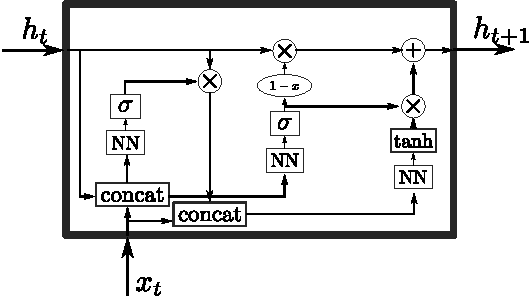
\includegraphics[width=0.6\textwidth]{figures/GRU.pdf}
	\end{figure}
\end{frame}



\begin{frame}{}{GRU}
	GRU blocks, or Gated Recurrent Units, are a type of recurrent neural network architecture that are similar to LSTMs in their function and ability to process sequential data. GRUs were introduced as a simplification of LSTMs, with the aim of reducing the number of parameters in the network and improving computational efficiency. GRUs achieve this by merging the forget and input gates in LSTMs into a single update gate, effectively combining the two operations in a single step.
	\vfill
	\begin{figure}
		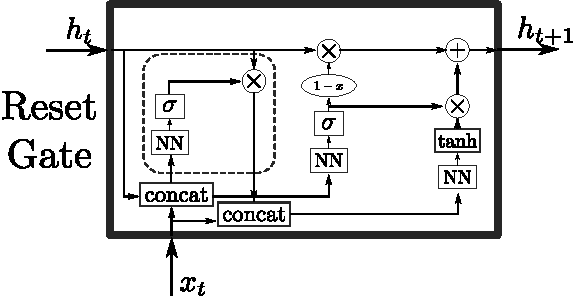
\includegraphics[width=0.6\textwidth]{figures/GRU_reset.pdf}
	\end{figure}
\end{frame}

\begin{frame}{}{GRU}
	GRU blocks, or Gated Recurrent Units, are a type of recurrent neural network architecture that are similar to LSTMs in their function and ability to process sequential data. GRUs were introduced as a simplification of LSTMs, with the aim of reducing the number of parameters in the network and improving computational efficiency. GRUs achieve this by merging the forget and input gates in LSTMs into a single update gate, effectively combining the two operations in a single step.
	\vfill
	\begin{figure}
		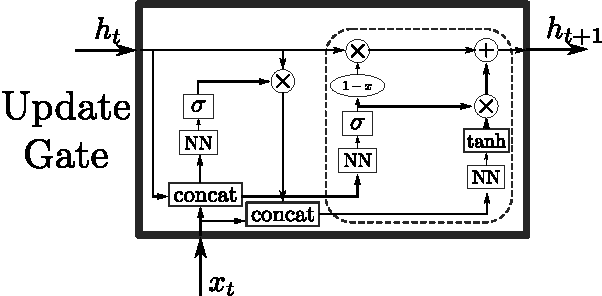
\includegraphics[width=0.6\textwidth]{figures/GRU_update.pdf}
	\end{figure}
\end{frame}

\begin{frame}

	Limitations of GRU RNNs:
	\begin{itemize}
		\item 	Computational complexity: GRUs are more computationally efficient than LSTMs but still more complex than feedforward neural networks.

		\item Long-term dependencies: GRUs may struggle with capturing long-term dependencies in sequences, although they perform better in this regard than vanilla RNNs.


		\item Vanishing gradient problem: GRUs can still be affected by the vanishing gradient problem that plagues all RNN models. This problem makes it difficult for the model to learn from long sequences.

		\item Non-stationary data: GRUs may struggle with nonstationary data, where the statistical properties of the data change over time.
	\end{itemize}
\end{frame}
\begin{frame}{}{Application of RNNs}
	Applications of RNNs:
	\begin{itemize}
		\item Natural language processing (NLP): Using RNNs for text classification, language translation, and text generation.
		\item Time-series prediction: Using RNNs to make predictions based on sequential data, such as stock prices and weather patterns.
		\item Speech recognition: Using RNNs for speech-to-text conversion.
	\end{itemize}
\end{frame}



\section{Transformer and Attention Mechanism}
\begin{frame}
	Transformers and Attention Mechanisms are recent advancements in deep learning, widely used for sequential data processing, especially in NLP. Unlike RNNs, which apply the same weights iteratively, Transformers leverage self-attention to dynamically assign importance to different sequence elements. This enhances their ability to capture long-range dependencies, improving NLP performance.
\end{frame}
\subsection{Self-Attention Mechanism}
\begin{frame}
	The self-attention mechanism in Transformers computes the importance of each token relative to others in a sequence. It generates a weighted representation where the most relevant tokens contribute more. Mathematically, self-attention is computed as:

	\[
		\mathrm{Attention}(Q, K, V) = \mathrm{Softmax}\left(\frac{QK^T}{\sqrt{d_k}} \right)V
	\]

	where \( Q \in \mathbb{R}^{m\times d_k} \), \( K \in \mathbb{R}^{n\times d_k} \), and \( V \in \mathbb{R}^{n\times d_v} \) are the query, key, and value matrices derived from the input sequence. The softmax function ensures proper weighting, producing the final representation.

\end{frame}
\begin{frame}
	\begin{columns}[c, onlytextwidth]
		\column{0.6 \textwidth}
		\textbf{Intuition behind the self-attention mechanism:}
		\begin{itemize}
			\item The \textbf{query} and \textbf{key} matrices measure the similarity between different tokens in the sequence.
			\item These similarity scores determine how much each \textbf{value} contributes to the final output.
			\item The resulting \textbf{weighted sum} of the values represents the output of the self-attention mechanism.
			\item This process captures the relationships between different parts of the input sequence, allowing the model to focus on the most relevant elements.
		\end{itemize}
		\column{0.4 \textwidth}
		\begin{figure}
			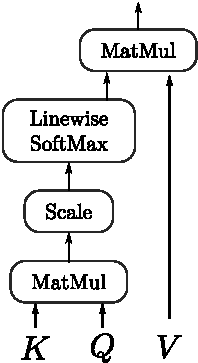
\includegraphics[width=0.6\textwidth]{figures/AttentionMech.pdf}
		\end{figure}
	\end{columns}
\end{frame}
\begin{frame}
	Illustration (source: \href{https://learnopencv.com/attention-mechanism-in-transformer-neural-networks/}{Understanding Attention Mechanism in Transformer Neural Networks}):
	\begin{figure}
		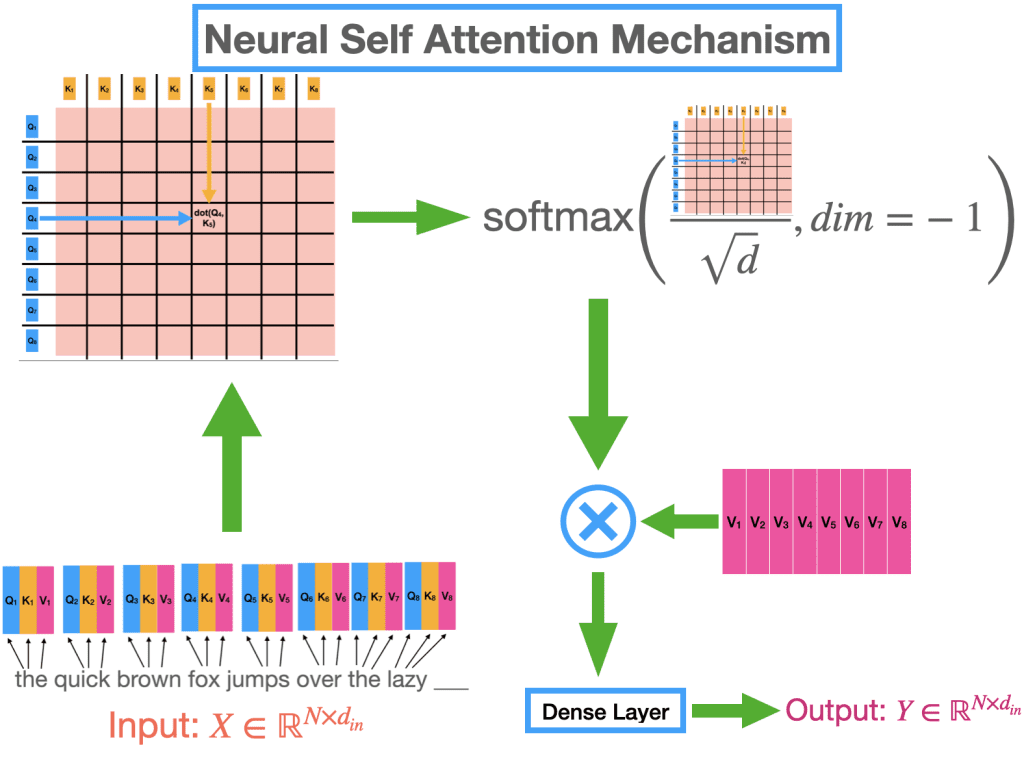
\includegraphics[width=0.5\textwidth]{figures/neural-self-attention-cover-picture-1024x767.png}
	\end{figure}
\end{frame}


\begin{frame}{}{Multi-Head Attention}
	\begin{columns}[c, onlytextwidth]
		\column{0.6 \textwidth}
		In Multi-head Attention, the self-attention mechanism is performed multiple times in parallel with different weight matrices, before being concatenated and once again projected, leading to a more robust representation of the input sequence. The intuition behind the three matrices ($Q$, $K$, $V$) remains the same as in self-attention, with $Q$ representing the query, $K$ the key and $V$ the value. Each head performs an attention mechanism on the input sequence, capturing different aspects and dependencies of the data, before being combined to form a more comprehensive representation of the input.
		\column{0.4 \textwidth}
		\begin{figure}
			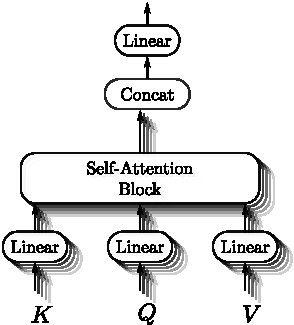
\includegraphics[width=0.8\textwidth]{figures/AttentionMechMulti.pdf}
		\end{figure}
	\end{columns}
\end{frame}

\begin{frame}{}{Visualizing Multi-Head Attention}
	\begin{columns}[c, onlytextwidth]
		\column{0.35 \textwidth}

		Visualizing Self-Attention for Image: \\
		\href{https://epfml.github.io/attention-cnn/}{Link}

		\column{0.65 \textwidth}
		\begin{figure}
			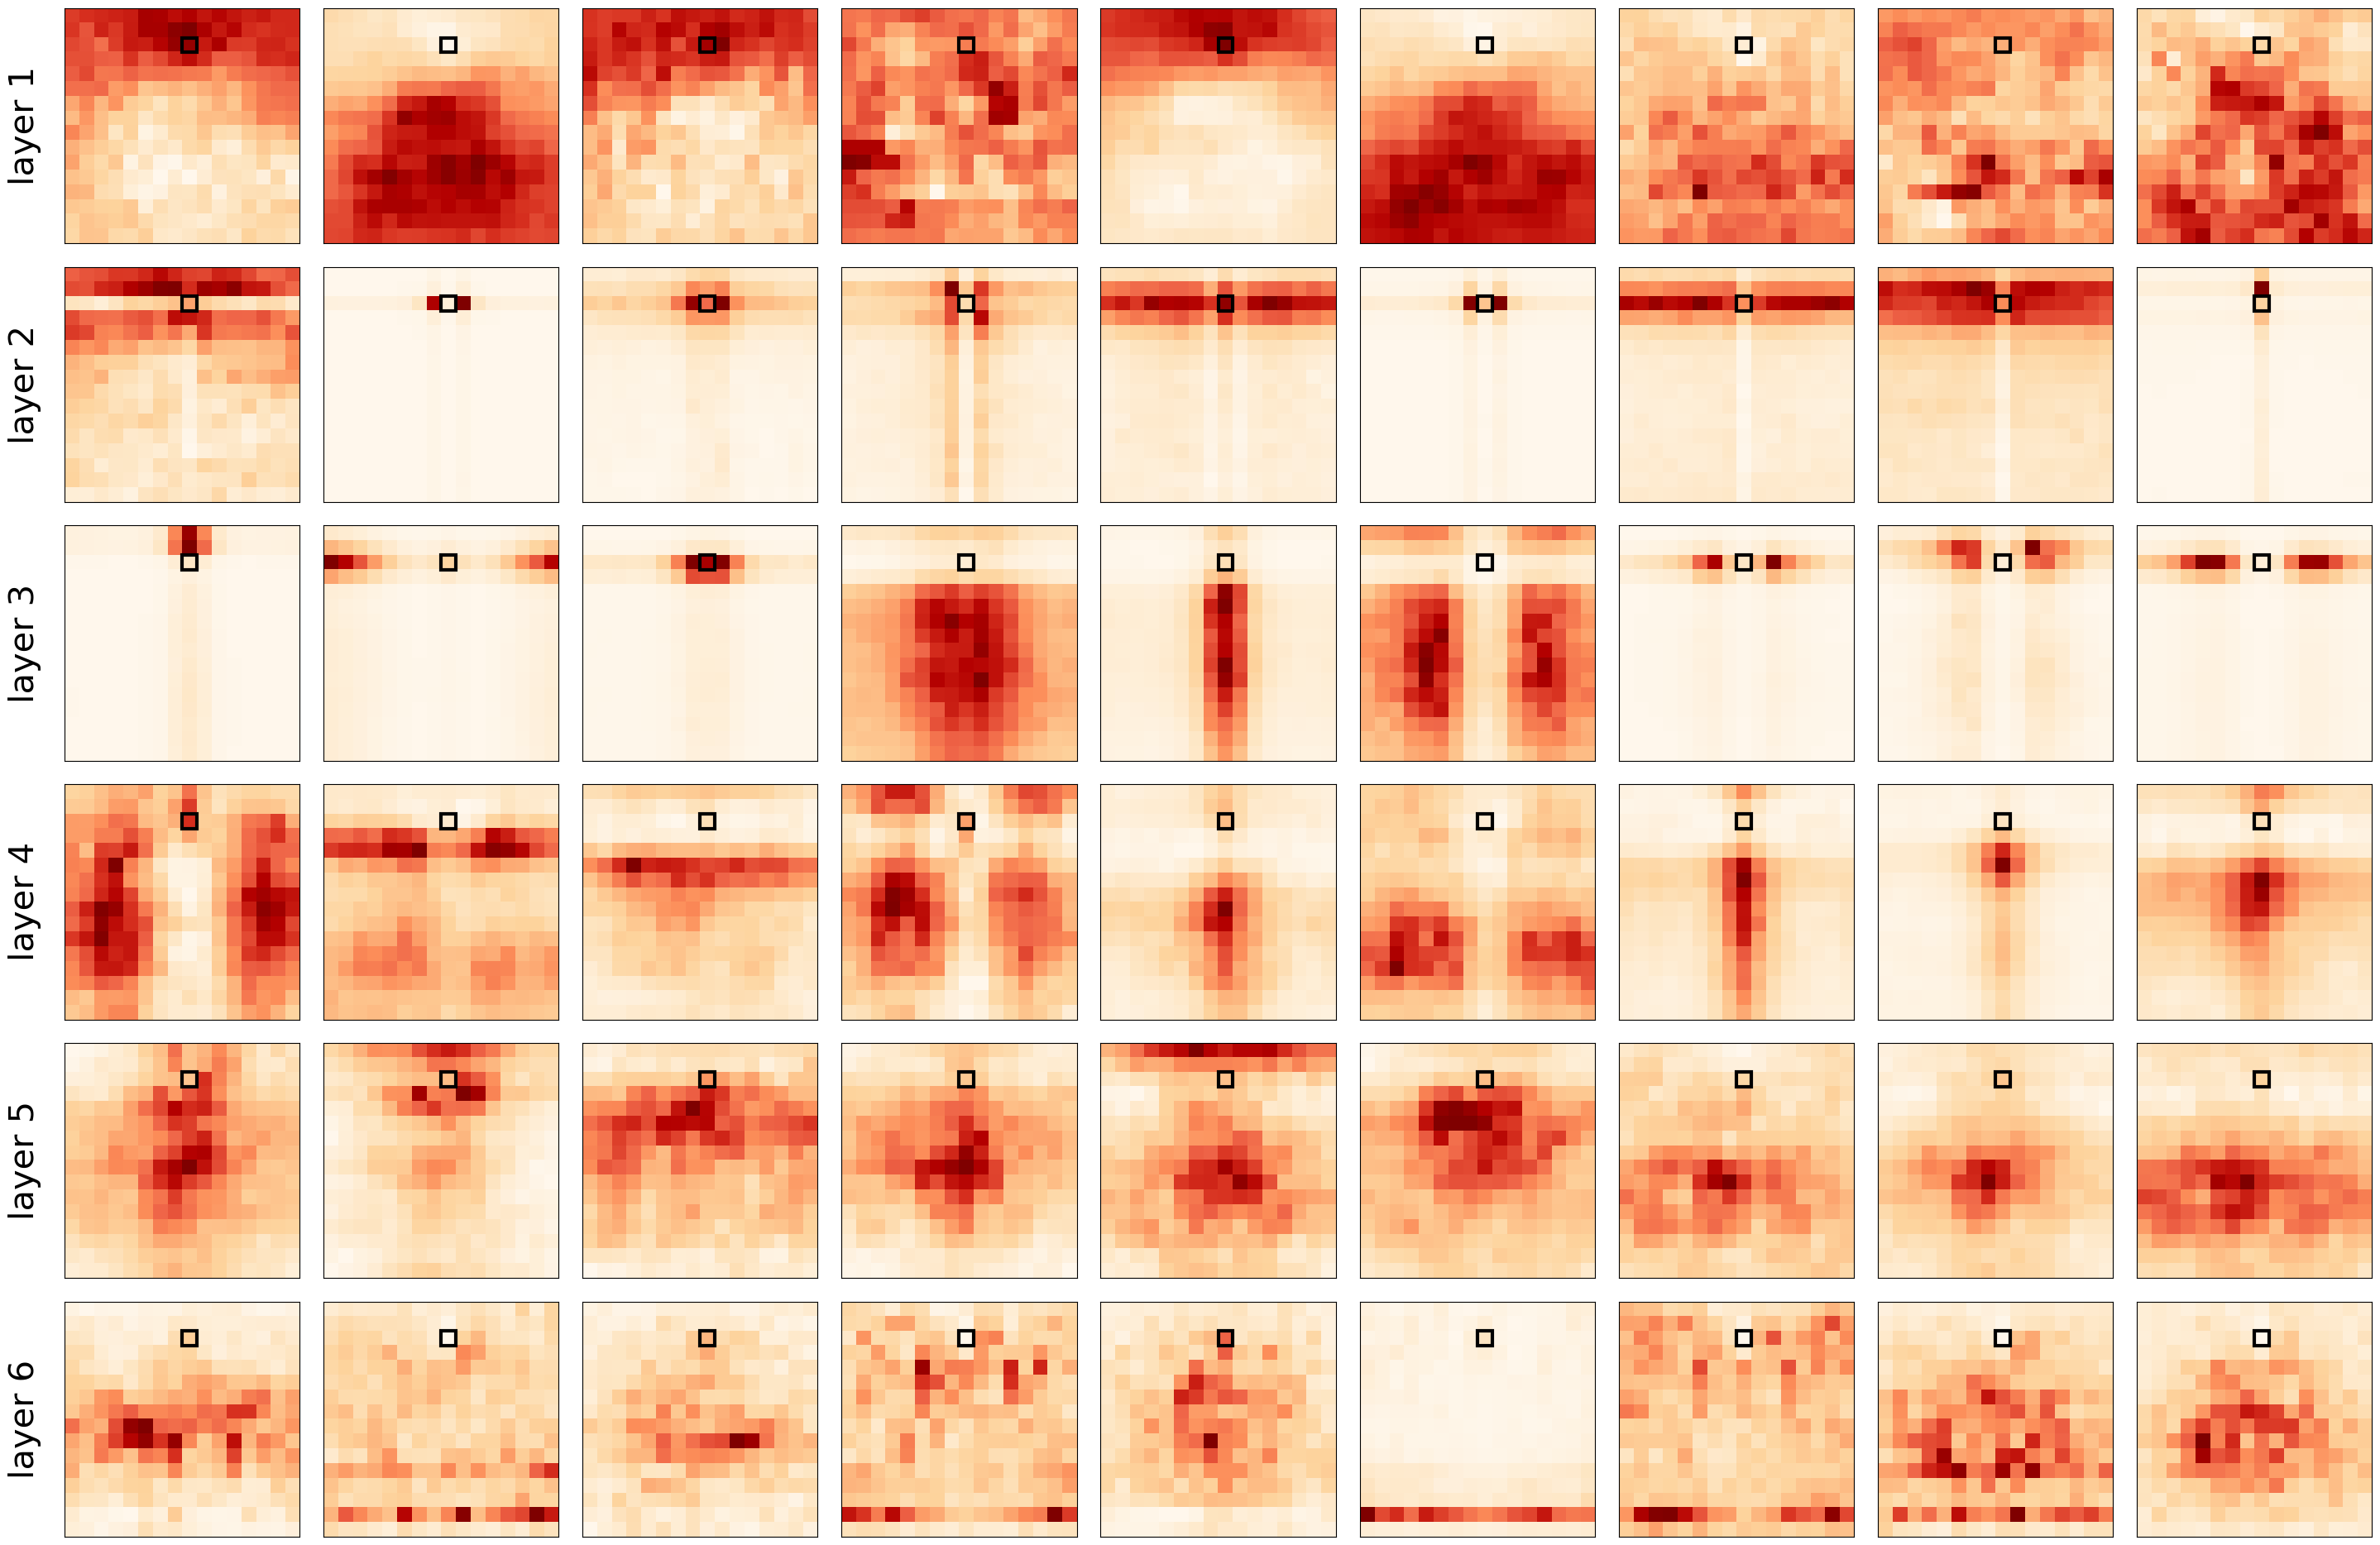
\includegraphics[width=0.8\textwidth]{figures/img_2_8.png}
		\end{figure}
	\end{columns}
\end{frame}

\subsection{Transformers Model}


\begin{frame}
	\begin{columns}[t, onlytextwidth]
		\column{0.6 \textwidth}

		Transformers are neural network models that use an encoder-decoder architecture. The encoder takes the input sequence and converts it into a continuous hidden representation, which is then passed to the decoder to generate the output sequence. The architecture of the transformer model is designed to allow the model to process the entire sequence in parallel, rather than processing one element at a time like in traditional RNNs.\newline

		Training of transformers involves optimizing a loss function that measures the difference between the model predictions and the true outputs. This loss function is usually based on the cross entropy between the predicted and true sequences.\newline

		The encoder-decoder mechanism is commonly referred to as the seq2seq mechanism.
		\column{0.05 \textwidth}
		\column{0.4 \textwidth}
		\begin{figure}
			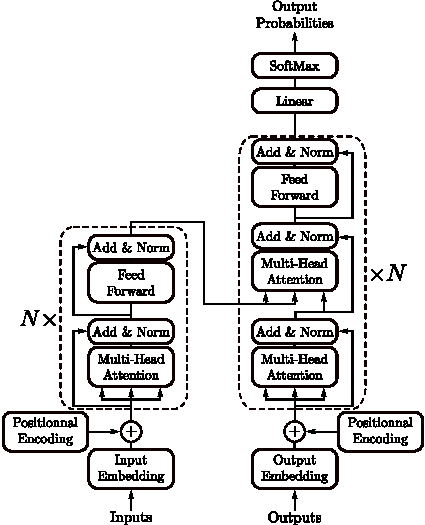
\includegraphics[width=0.9\textwidth]{figures/transformers.pdf}
		\end{figure}
	\end{columns}

\end{frame}

